\begin{center}
\textsc{\Large Laboratorio 2}~\\
{\large Videojuegos, Programación, Diseño}~\\
\emph{Cámaras Virtuales}
\end{center}

\section{Pre-Laboratorio}
\begin{itemize}
\item Investigar:
\begin{enumerate}
  \item Vídeo juegos en primera persona.
  \item Vídeo juegos en tercera persona.
  \item Side-scrollers.
  \item Perspectiva.
  \item Proyección Ortogonal.
  \item Géneros de videojuegos.
\end{enumerate}
\item Investigar según su framework, biblioteca o motor de juego escogido.
\begin{enumerate}
	\item Implementación de cámaras en el juego.
	\item Manejo de escenas.
	\item Scripting o programación de la lógica de juego.
\end{enumerate}
\end{itemize}
\section{Definición}
En los videojuegos se utilizan cámaras virtuales para mostrar un mundo 3D o 2D en algún dispositivo visual. Un sistema virtual de cámaras se encarga de controlar una o mas cámaras en un escenario de juego. Usualmente la cámara en muchos frameworks y bibliotecas para desarrollo de videojuegos no es mas que otro objeto en escena \cite{fund_gamedesign}.
\section{Conceptos}
\begin{wrapfigure}[7]{l}{0.3\linewidth}
\includegraphics[width=\linewidth]{media/frustum.eps}
\caption{\emph{Viewing Frustum} de una cámara virtual donde se muestra el far y near clipping plane \cite{microsoft_frustum}.}
\label{fig:frustum}
\end{wrapfigure}
Algunos conceptos necesarios para entender el uso de cámaras en la gran mayoría de los frameworks, bibliotecas y motores para el desarrollo de videojuegos \cite{unity_camera}.
\subsection{Tipos de Proyección}
Existen dos tipos proyección en la mayoría de los frameworks y bibliotecas para el desarrollo de videojuegos estos son proyección perspectiva y proyección ortogonal.
\subsubsection{Perspectiva}
\setlength\intextsep{0pt}
\begin{wrapfigure}[6]{r}{0.3\linewidth}
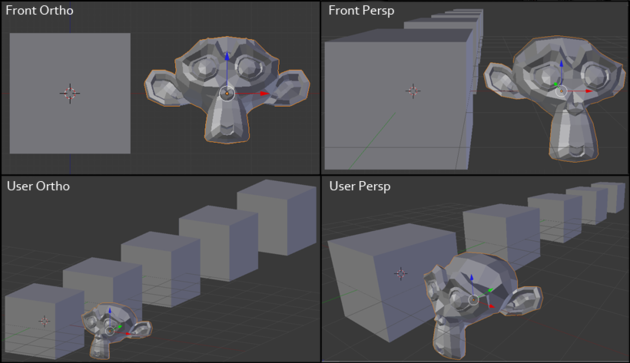
\includegraphics[width=\linewidth]{media/projections.png}
\caption{Proyección ortogonal y perspectiva.}
\end{wrapfigure}
Es la forma natural en que el ojo humano percibe una escena, en la proyección perspectiva los objetos distantes se ven mas pequeños que los objetos cercanos dando profundidad a distintos objetos en una escena. Este tipo de proyección es utilizada usualmente en juegos 3D.
\subsubsection{Ortogonal}
En una proyección perspectiva un objeto lejano es mas pequeño que un objeto cercano, en proyección ortogonal se ignora este efecto, eliminando la profundidad de escena. Este tipo de perspectiva es utilizada en muchos juegos 2D.
\subsection{Field Of View (FoV) o Campo de Vista}
\label{subsec:fov}
Es el ancho del angulo de vista de la cámara, indica la extension de lo puede ver la cámara en cualquier momento, usualmente se mide en ángulos, este angulo puede ser el field of view vertical o el field of view horizontal dependiendo del framework, biblioteca o motor de juego usado (ver \ref{fig:camera}) \cite{feng_fovy}.
\subsection{Clipping Planes o Planos de Clipping}
\label{subsec:clipping_planes}
En computación se manejan términos discretos por lo tanto una cámara no puede ver hacia el infinito, para esto están el far y near clipping planes los cuales indican donde termina el renderizado de escena y donde empieza según la posición de la cámara respectivamente (ver \ref{fig:frustum} y \ref{fig:camera}).
\subsubsection{Near Clipping Plane o Plano de Clipping Cercano}
Es donde empieza a dibujarse los objetos de escena en display, los objetos antes de este punto son ignorados por el motor gráfico.
\subsubsection{Far Clipping Plane o Plano de Clipping Lejano}
Es donde termina de dibujarse los objetos de escena en display, los objetos mas lejanos a este punto son ignorados por el motor gráfico.
\begin{figure}[H]
\centering
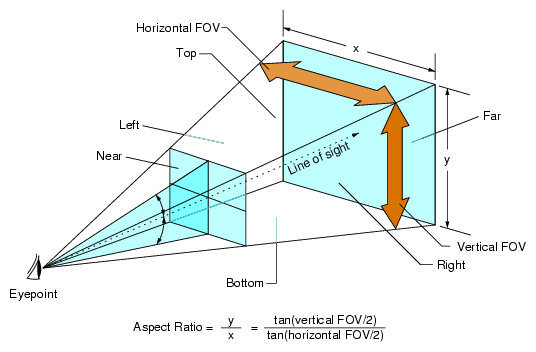
\includegraphics[width=0.9\linewidth]{media/camera.png} 
\caption{Parámetros de una Cámara Virtual}
\label{fig:camera}
\end{figure}
\newpage
\section{Tipos de Sistemas de Cámara en Videojuegos}
Existen principalmente tres tipos de sistemas de cámara en videojuegos. En un sistema \emph{fixed} la cámara no cambia sus parámetros originales, un sistema \emph{tracking} sigue algún objeto en juego, y un sistema \emph{interactive} la cámara es parcialmente autónoma y cambia sus parámetros según distintas situaciones. Para implementar distintos sistemas de cámara los desarrolladores de videojuegos usan técnicas como programación con restricciones o inteligencia artificial. 
\subsection{Estáticas (\emph{Fixed})}
\begin{wrapfigure}[9]{l}{0.4\linewidth}
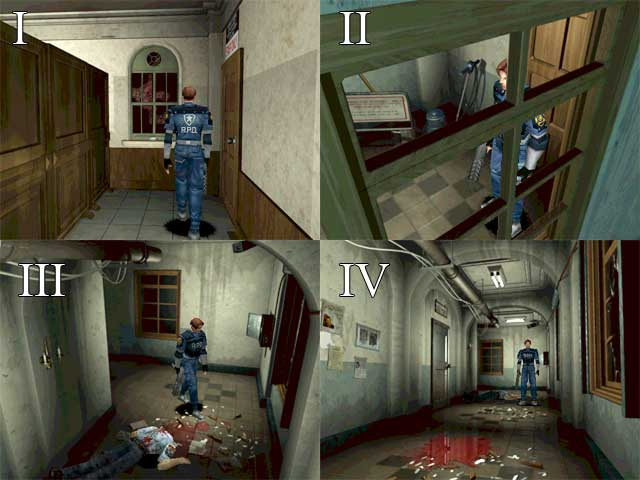
\includegraphics[width=\linewidth]{media/resident_evil_camerawork.jpg} 
\caption{Ejemplo de cámaras estáticas en \emph{Resident Evil 2} \cite{fixed_camera} \cite{residentevil2}.}
\end{wrapfigure}
En este tipo de cámara las propiedades de la cámara como su posición, orientación y campo visual (\emph{field of view}) son colocadas durante el desarrollo del juego y estas no cambian durante el \emph{gameplay}. Algunos ejemplos de juegos con este tipo de camara son los primeros Resident Evil, y Alone In The Dark, usualmente es utilizada para crear tension \cite{res5_review}\cite{fixed_camera}.
\subsection{Seguidoras (\emph{Tracking})}
Este tipo de cámara sigue a algún objeto en el juego usualmente el personaje principal u otro objeto de considerable importancia. Este sistema presenta varios problemas sobretodo en ambientes tridimensionales y tercera persona donde la cámara podría quedar detrás de una objeto que ocluye totalmente la vista o no deja ver algún objeto de interés al jugador \cite{fund_gamedesign}. Su uso es muy común en los primeros juegos 3D en tercera persona como \emph{Crash Bandicoot} \cite{crashbandicoot} o \emph{Tomb Raider} \cite[p.~39]{bobbatesgamedesign}, los juegos primera persona también utilizan una cámara seguidora, a diferencia de en tercera persona donde la cámara esta detrás del personaje en un juego primera persona la cámara esta como visión del personaje principal, en los juegos 2D esta cámara esta presente en todos los juegos tipo side-scroller.
\newpage
\subsection{Interactivas (\emph{Interactive})}
\begin{wrapfigure}[11]{r}{0.4\linewidth}
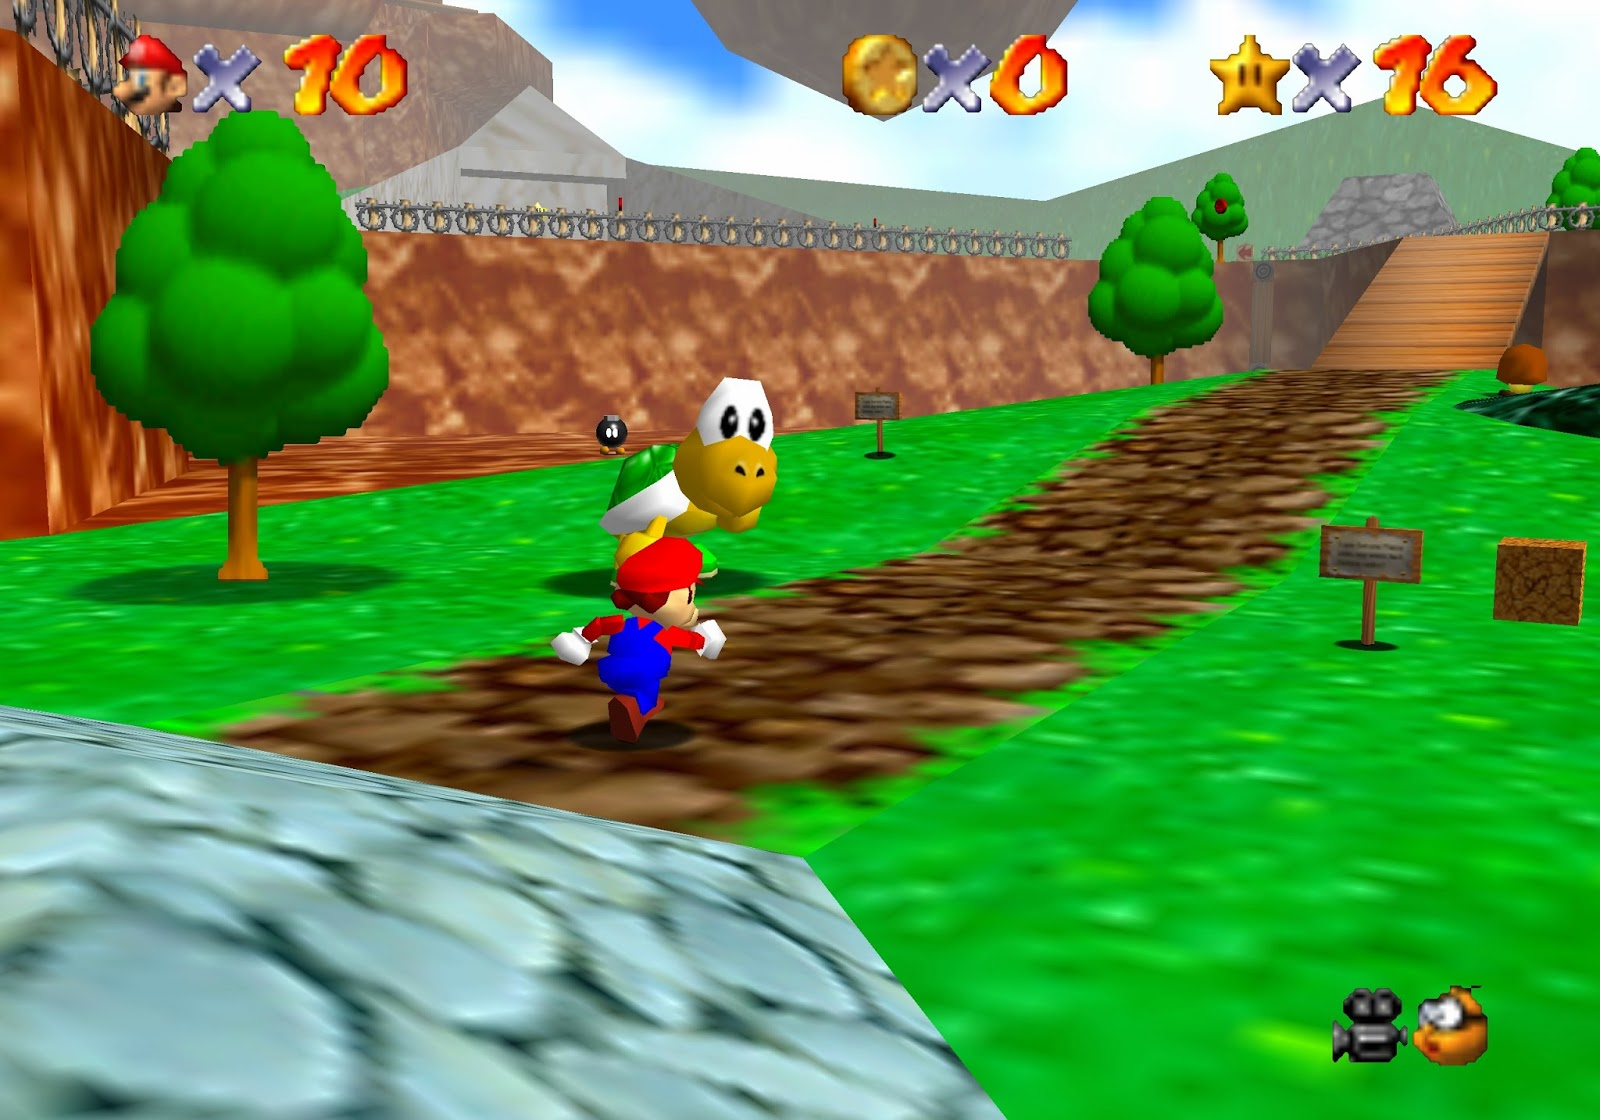
\includegraphics[width=\linewidth]{media/supermario64.jpg} 
\caption{En \emph{Super Mario 64} la cámara rota de forma inteligente para mostrar el camino \cite{supermario64}.}
\end{wrapfigure}
Las cámaras interactivas son cámaras que cambian su posición, campo visual u orientación según distintas situaciones, lugares o intereses del juego y sus desarrolladores, usualmente estas cámaras poseen alguna forma de inteligencia artificial. En su mayoría las cámaras interactivas son cámaras tracking mejoradas, estas siguen al personaje como lo hace una cámara tracking pero su posición y orientación puede cambiar si estas se ven obstruidas por algún objeto o cambian sus parámetros para mostrar objetos de interés claramente evitando de esta forma las desventajas principales de una cámara tracking. Algunos ejemplos de juegos con este tipo de camara son \emph{Super Mario 64}, \emph{Super Mario Sunshine}, \emph{The Legend of Zelda: The Wind Waker.}
\section{Actividad}
\begin{itemize}
\item Durante esta actividad se creara la base del proyecto y se implementara inicialmente la cámara según el diseño de su juego. Los objetivos de la actividad son:
\begin{enumerate}
  \item Crear una pequeña escena con \emph{placeholders} \footnote{Un \emph{placeholder} no es mas que un procurador de un objeto, de manera que el \emph{placeholder} es remplazado en un futuro por el objeto real.}.
  \item Implementar la cámara principal de juego según el diseño del juego.
  \item Debe crear una estructura de datos (ejemplo una clase) que defina a los actores principales en su mundo de juego, incluyendo el jugador principal. Esto depende directamente del diseño del juego.
  \item Debe asociar esta estructura a un \emph{placeholder} que representa cada actor, incluyendo el jugador principal.
  \item Agrege en la lógica de juego (esto se realiza usualmente a través de scripts u otro medio que provea las herramientas que eligió) comportamientos a uno o varios actores en escena, este comportamiento debe ser observable por la cámara.
\end{enumerate}
\end{itemize}

\subsection{Ejemplo en Unity3D}
En esta sección se muestra como ejemplo la realización de la actividad del laboratorio en Unity3D, según su herramienta de trabajo algunas cosas puede ser muy parecidas o muy diferentes por esto es recomendado en el pre-laboratorio investigar sobre su herramienta de trabajo igualmente en la actividad del laboratorio 1 se sugieren algunos parámetros para escoger su herramienta. Para esto usaremos el motor de juego Unity v5.0.

Luego de descargar, instalar el motor de juego Unity3D (en el laboratorio 1 se encuentran los distintos links para cada motor y framework recomendado) para empezar un juego primero tenemos que crearlo, para esto ejecutamos \emph{Unity.exe} normalmente encontrado en \emph{[Carpeta de Instalacion]/Editor/Unity.exe} y creamos un nuevo proyecto dando click sobre \emph{New Project}.\\~

\begin{figure}[H]
\centering
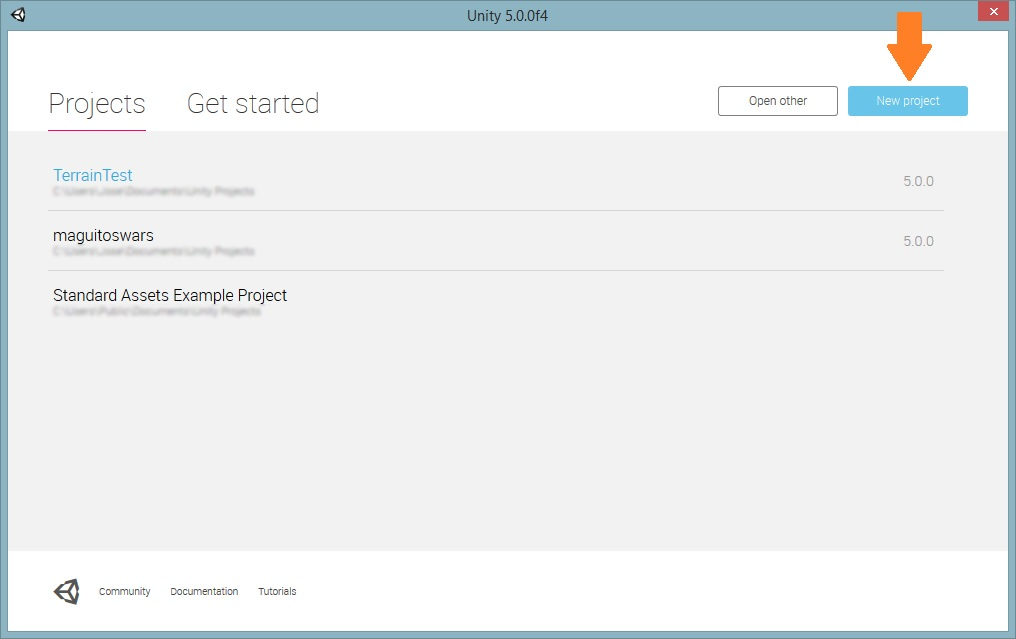
\includegraphics[width=0.80\linewidth]{media/1_ss1.jpg} 
\label{fig:unity_1}
\end{figure}

Luego se debe colocar el nombre del proyecto de juego (1), seleccionar entre Unity 3D o 2D (2) en nuestro caso seleccionaremos 2D ya que el juego a realizar durante este laboratorio general debe ser 2D, sin embargo se puede crear también juegos 2D en modo Unity 3D utilizando proyección ortogonal para la camara y finalmente debemos crear el proyecto dando click sobre \emph{Create Project} (3).\\~

\begin{figure}[H]
\centering
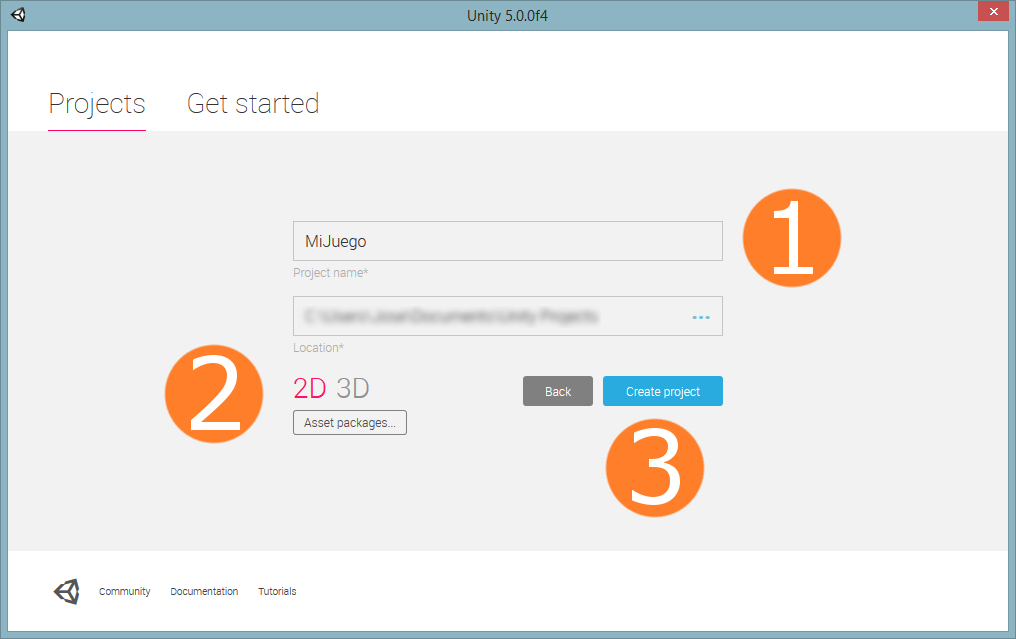
\includegraphics[width=0.80\linewidth]{media/1_ss2.jpg} 
\caption{Nombre del juego (1), Modo 2D o 3D (2), Crear Proyecto (3)}
\label{fig:unity_2}
\end{figure}

Esto nos lleva directamente al editor de escena en Unity, la terminología utilizada para describir las distintas partes de la interfaz del motor de juego suele cambiar entre motores. En el caso de Unity al iniciar por primera vez nos muestra la interfaz por defecto donde podemos ver la jerarquía de los objetos de escena en el panel izquierdo, las propiedades del objeto actualmente seleccionado en el panel derecho, el explorador de archivos del proyecto en el panel inferior y la escena en el centro como foco principal. Para desplazarse en escena puede usar click derecho y central sostenido y las teclas direccionales.\\~

\begin{figure}[H]
\centering
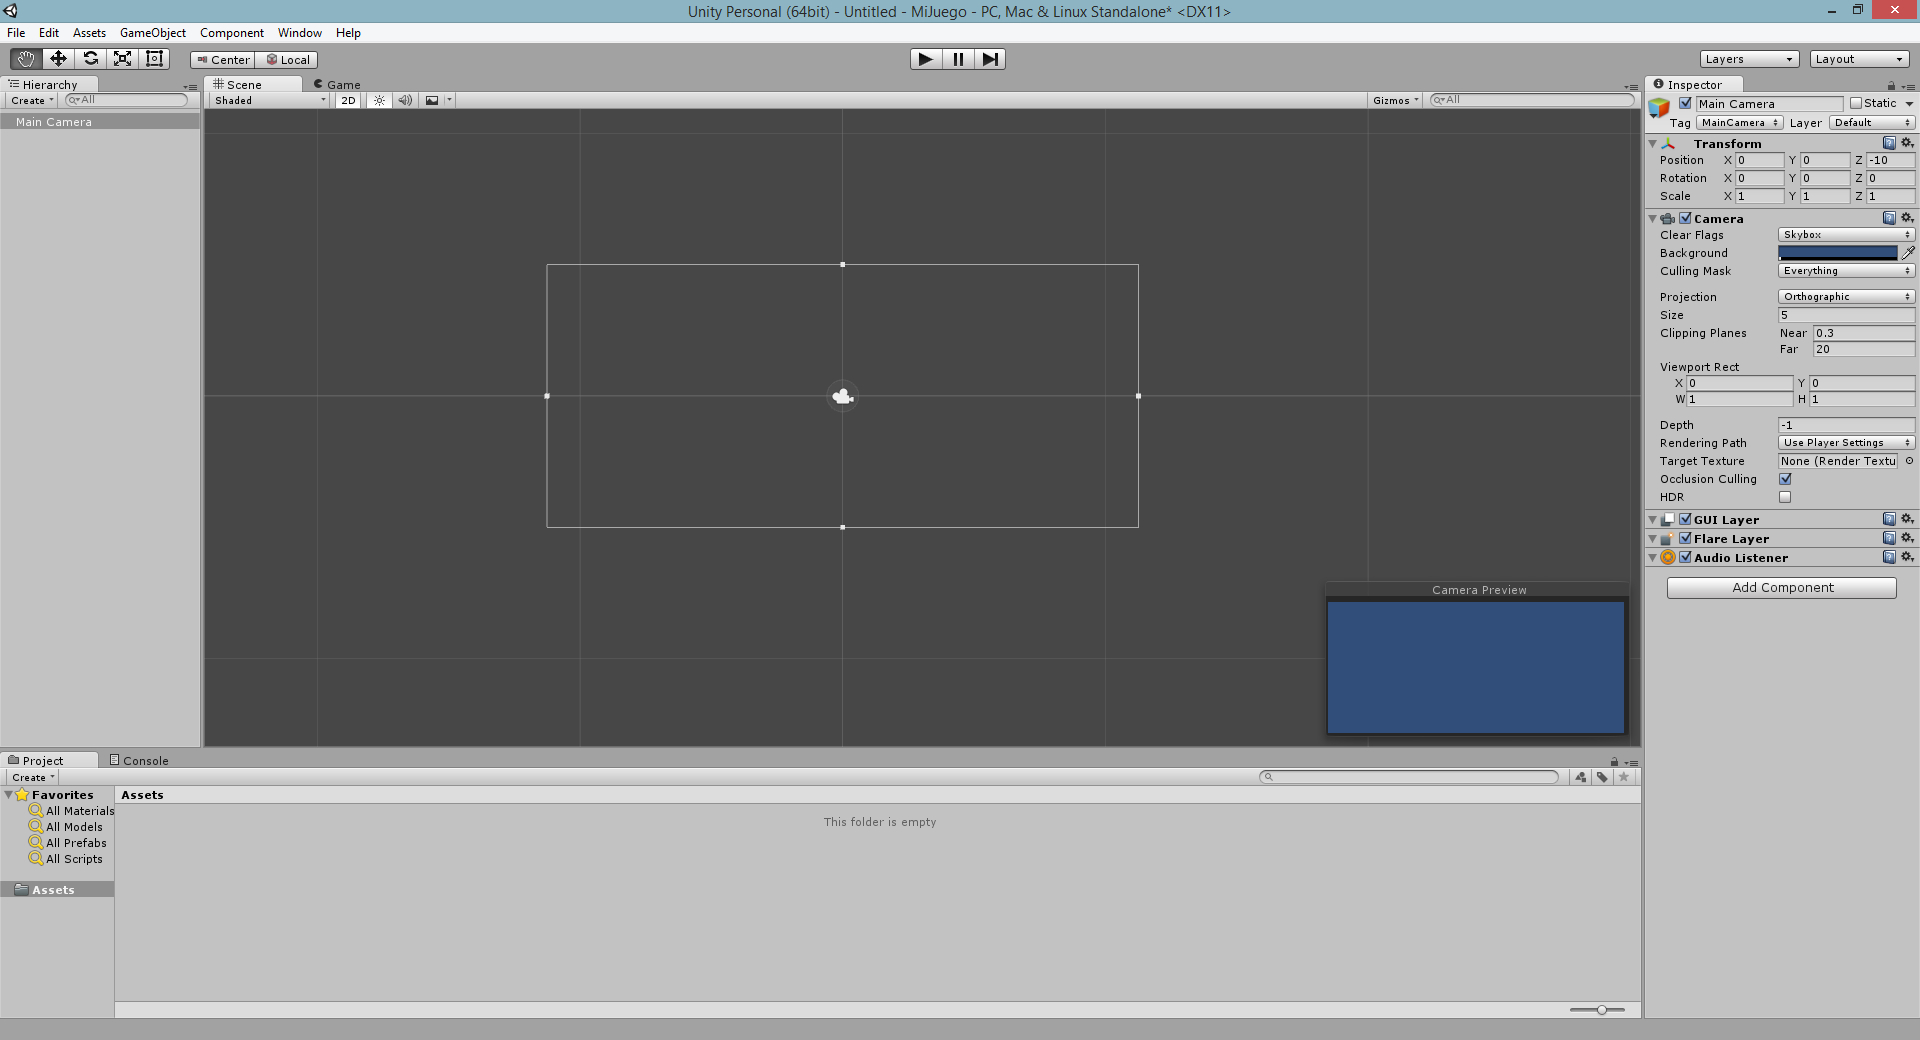
\includegraphics[width=0.80\linewidth]{media/1_ss3.jpg} 
\label{fig:unity_3}
\end{figure}

Por defecto Unity nos crea una cámara como objeto de escena al iniciar un proyecto, esta con proyección ortogonal para modo 2D y perspectiva para modo 3D, vamos a eliminar este objeto de escena y crear una cámara por nuestra cuenta. Para eliminar la cámara damos click derecho sobre \emph{Main Camera} en la jerarquía de objetos (panel izquierdo) y click sobre \emph{Delete}.

Para crear un objeto en escena de tipo cámara en Unity debemos ir a Menu de Herramientas (arriba), dar click sobre \emph{Game Object} y luego en \emph{Camera} (1).\\~

\begin{figure}[H]
\centering
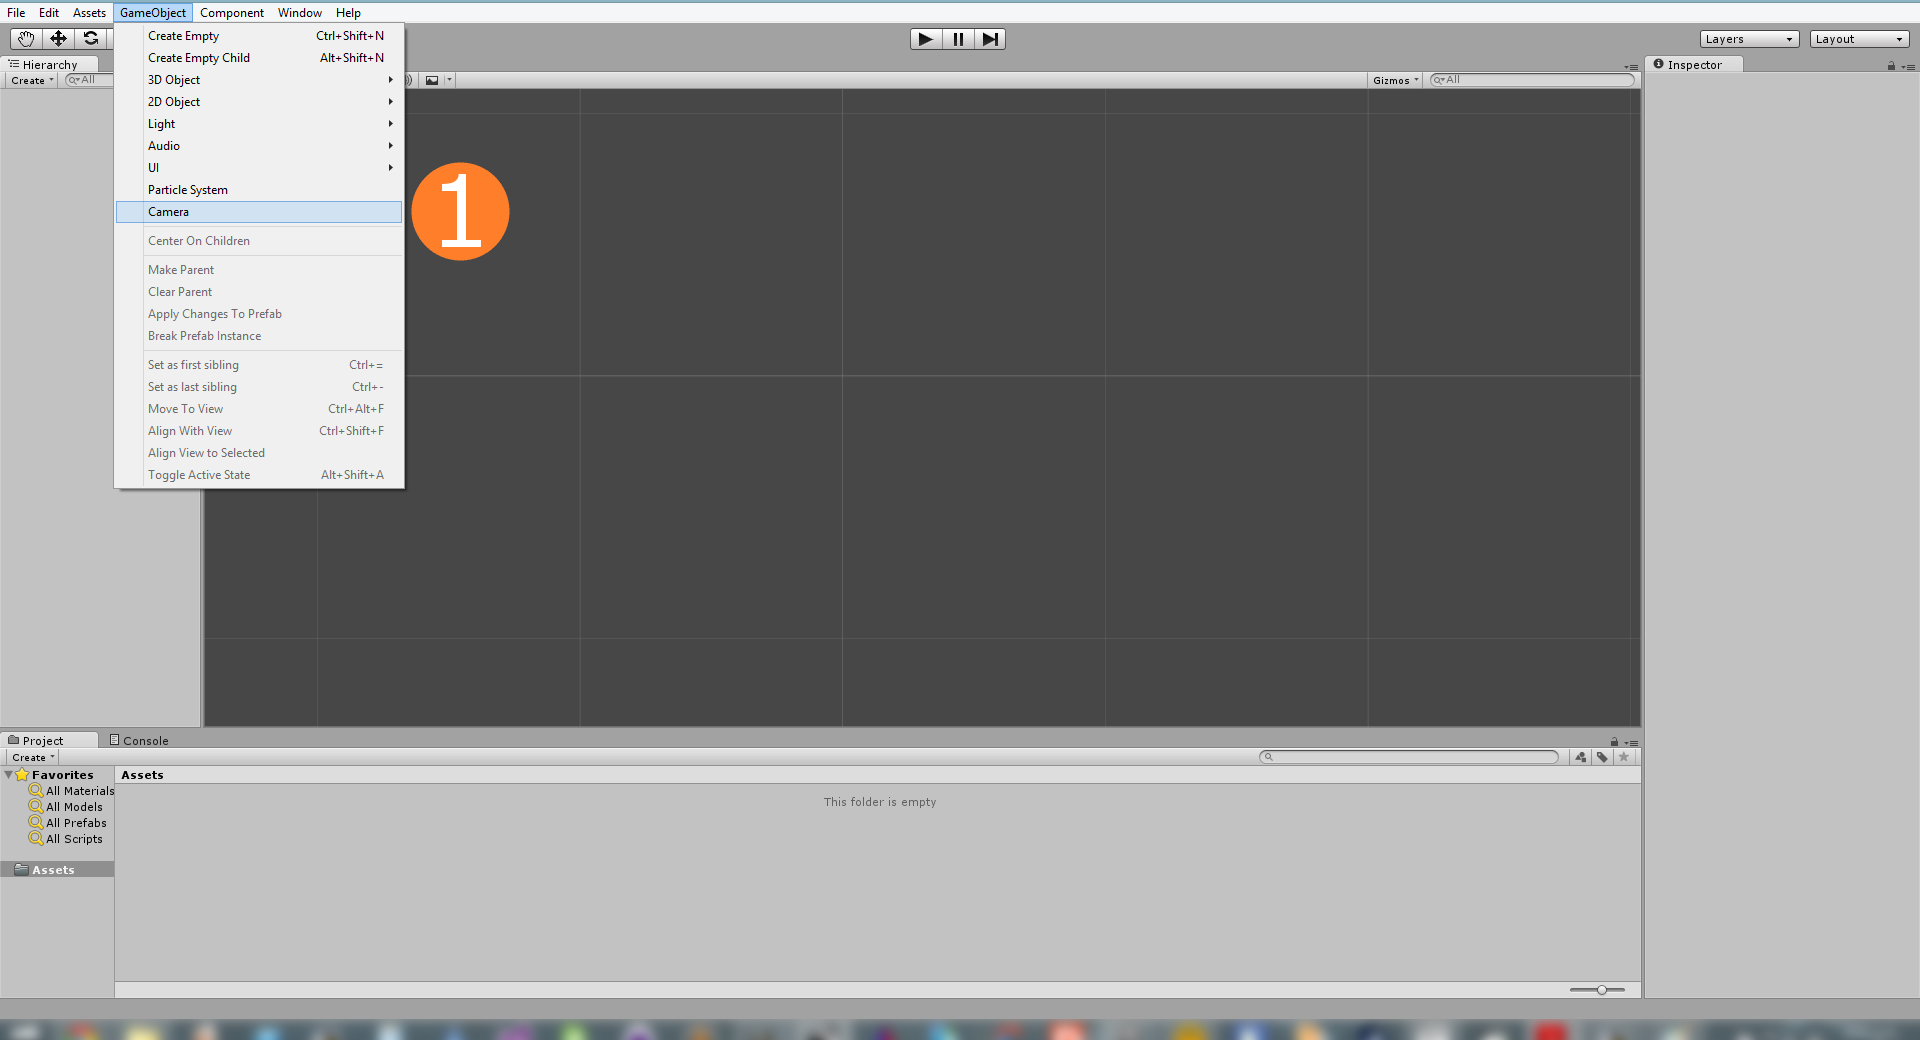
\includegraphics[width=0.80\linewidth]{media/1_ss4.jpg} 
\label{fig:unity_4}
\end{figure}

Por defecto la cámara es creada con proyección perspectiva, podemos cambiar esto a conveniencia, dando click sobre el nuevo objeto \emph{Camera} creado (1) en las propiedades de objeto (panel izquierdo) podemos cambiar el tipo de proyección a perspectiva u ortogonal (perspective y orthographic) entre otras cosas como la distancia de los clipping planes (Sección \ref{subsec:clipping_planes}), posición de la cámara, rotación de la cámara, tamaño de la ventana de vista (Viewport Rect), tamaño para proyección ortogonal, campo de visión (Sección \ref{subsec:fov}) para proyección perspectiva, etc (4). Si damos click sobre el botón \emph{2D} (2) en el editor de escena intercambiar entre ver la escena en 2D o 3D, en modo 2D con la cámara seleccionada es fácil observar el volumen de la vista de la cámara (3).

\begin{figure}[H]
\centering
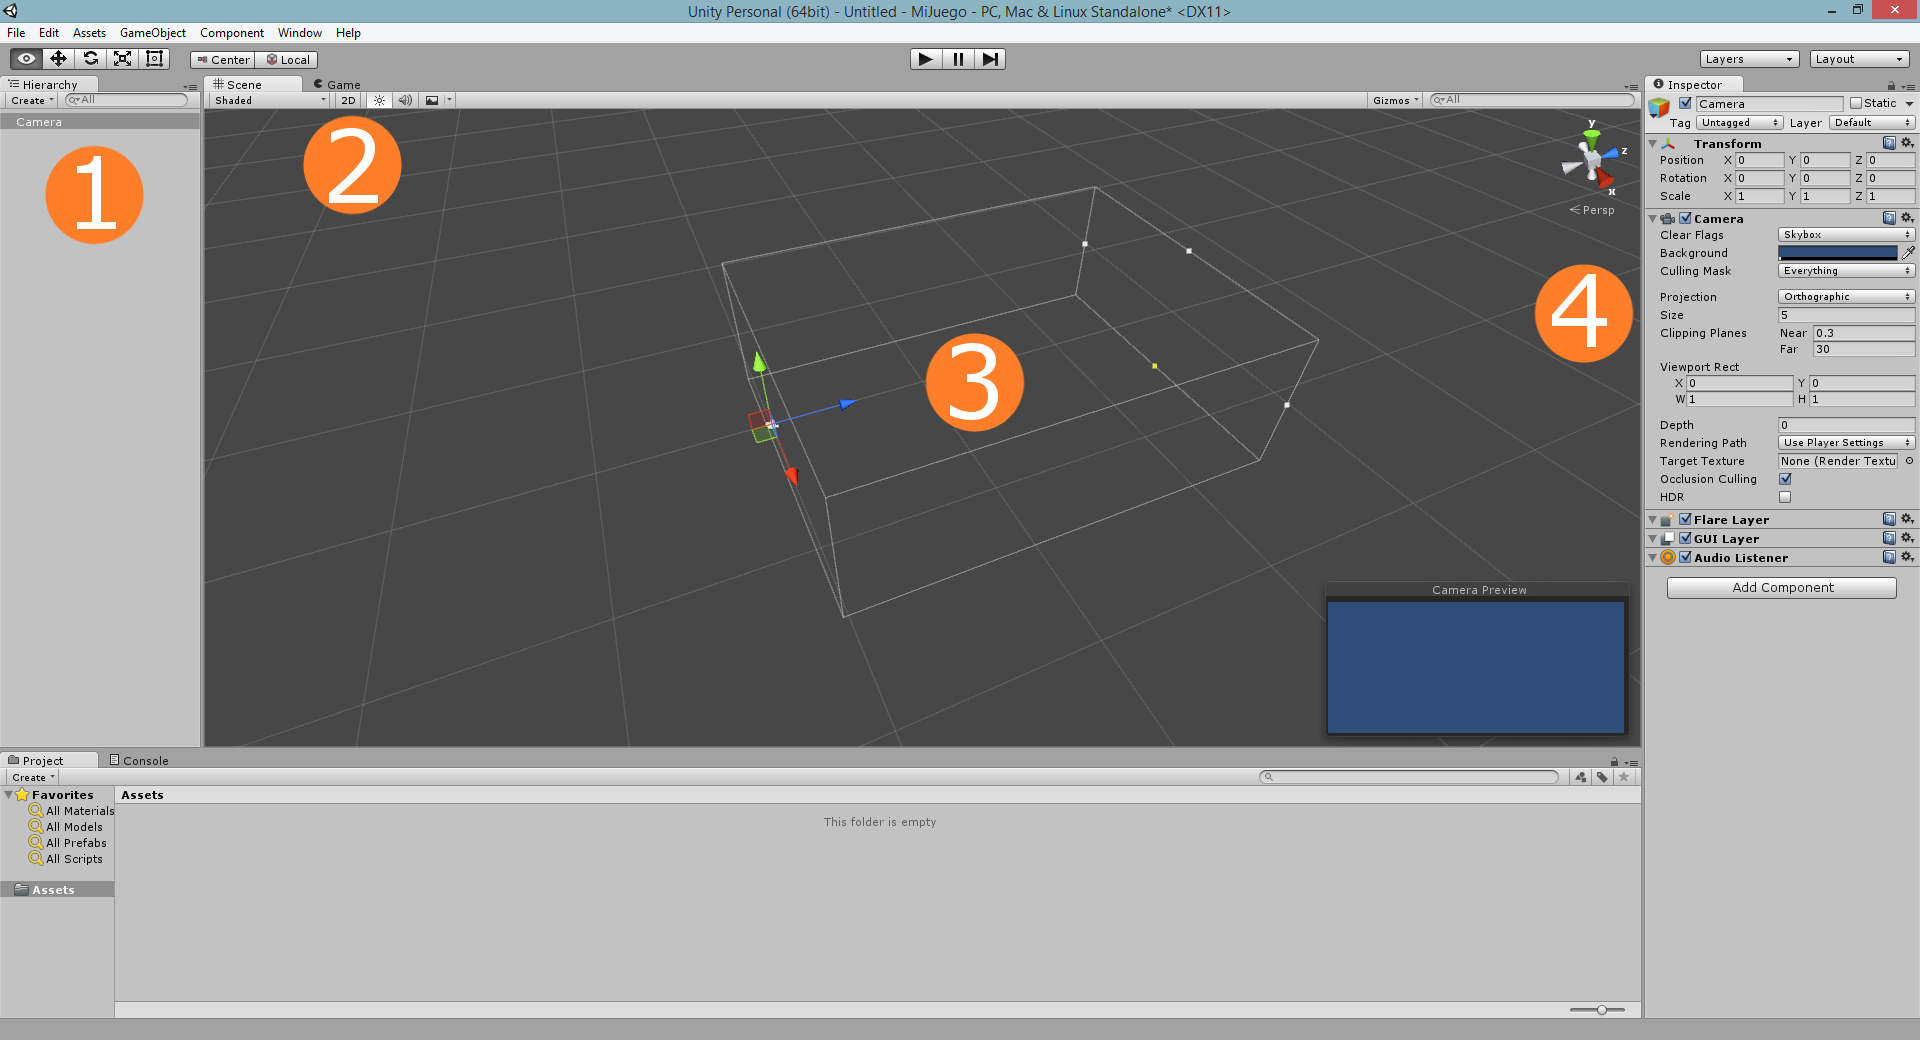
\includegraphics[width=0.80\linewidth]{media/1_ss5.jpg} 
\label{fig:unity_5}
\end{figure}

Igualmente como creamos la cámara vamos crear objetos placeholder para representar el jugador principal, actores y ambiente en distintas posiciones y tamaños, solamente que esta vez en vez de cámaras vamos a crear \emph{2D Object $\rightarrow$ Sprite} y \emph{3D Object} (1). Cada objeto es recomendado nombrarlos adecuadamente (2) y categorizarlos (en Unity esto se hace con el uso de \emph{Tags}). Para los sprite usaremos en propiedades \emph{Sprite} alguno por defecto o se puede usar alguno importado (3) por \emph{Assets $\rightarrow$ Import New Asset} (estos deben ser imágenes en este caso) y en \emph{Color} alguno de preferencia para diferenciar, recordemos que estos son placeholders.\\~

\begin{figure}[H]
\centering
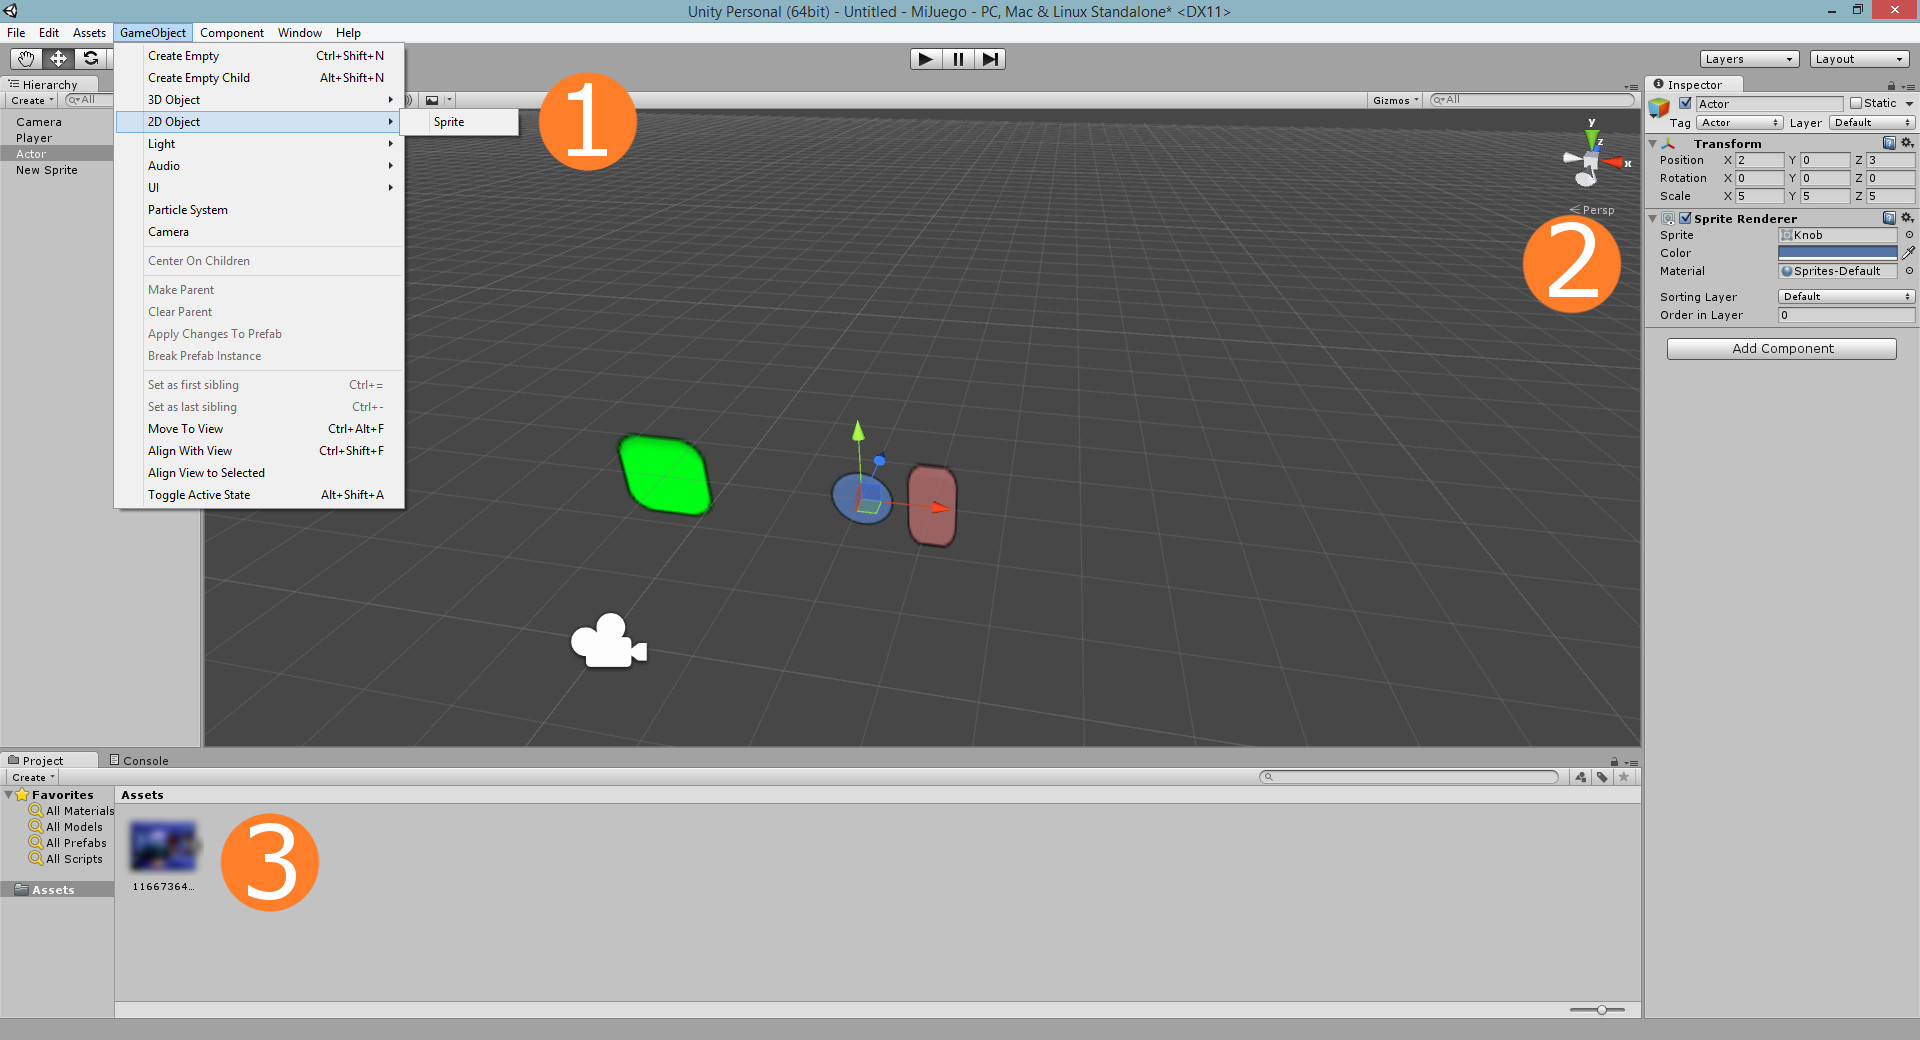
\includegraphics[width=0.80\linewidth]{media/1_ss6.jpg} 
\label{fig:unity_6}
\end{figure}

Vamos a crear ahora scripts asociados a cada uno de estos objetos, estos scripts en un futuro contendrán distintas propiedades, comportamientos y recursos asociados a estos objeto, en Unity un objeto puede tener asociado un numero indefinido de scripts. Para asociar un script a un objeto seleccionamos este objeto, en la barra de herramientas (arriba) damos click sobre \emph{Component $\rightarrow$ Add...} (1) esto abre un menú desplegable sobre las propiedades del objeto, seleccionamos \emph{New Script} (2) y colocamos un nombre apropiado, Unity agrega estos scripts a los \emph{Assets} del proyecto (3).\\~

\begin{figure}[H]
\centering
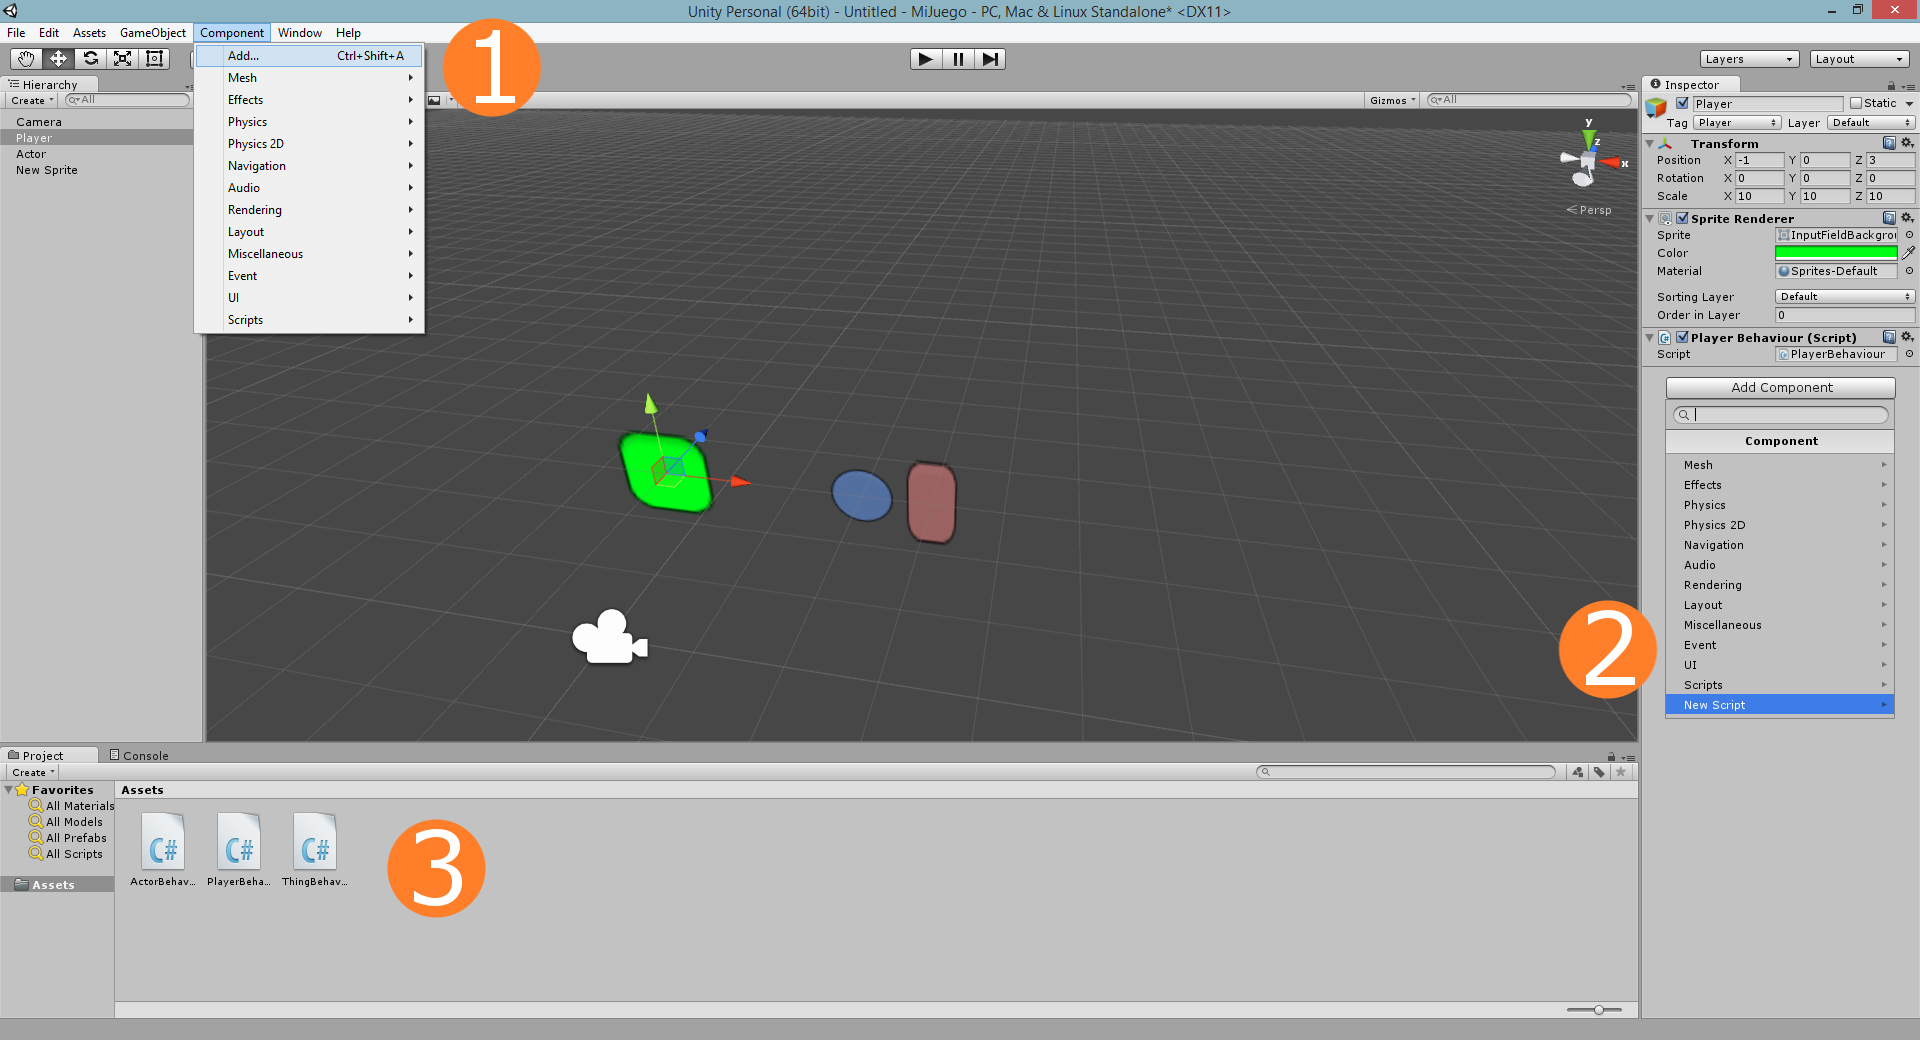
\includegraphics[width=0.80\linewidth]{media/1_ss7.jpg} 
\label{fig:unity_7}
\end{figure}

Para editar estos scripts Unity trae un editor por defecto llamado MonoDevelop, sin embargo se puede usar otros editores externos para modificar los scripts, una de las ventajas de MonoDevelop es que se puede compilar el proyecto desde el mismo editor, sin embargo existen plugins para otros editores como Visual Studio que permiten esto. El formato por defecto de los scripts en C\# en Unity es el siguiente.\\~

\lstset{language=[Sharp]C}
\begin{lstlisting}
using UnityEngine;
using System.Collections;
public class PlayerBehaviour : MonoBehaviour {
	// Use this for initialization
	void Start () {}	
	// Update is called once per frame
	void Update () {}
}
\end{lstlisting}

Unity importa por defecto \emph{UnityEngine} y las estructuras en \emph{System.Collections}, el template presenta dos procesos \emph{Start} y \emph{Update}. \emph{Start} se ejecuta cuando se crea las instancia del objeto asociado al script. \emph{Update} se ejecuta por cada frame. Agreguemos propiedades al objeto \emph{Player} a través del script, en este caso agreguemos un parámetro de vida (\emph{Health}) y velocidad (\emph{Speed}).\\~

\begin{lstlisting}
public class PlayerBehaviour : MonoBehaviour {
	public float Health = 100.0f;
	public float Speed = 10.0f;
	// Use this for initialization
	void Start () {}	
	// Update is called once per frame
	void Update () {}
}
\end{lstlisting}

Esta propiedad debe aparecer en el componente \emph{Script} asociado al objeto \emph{Player} ya que estos son públicos. Uno de los objetivos de la actividad es realizar ciertas acciones sobre algún objeto de manera que esto sea notable por la cámara. Hagamos entonces en el script que el jugador se mueva entre dos puntos constantemente, para esto debemos modificar la transformada del objeto, la transformada posee información de la posición, rotación y escala del objeto asociado al script.\\~

\begin{lstlisting}
public class PlayerBehaviour : MonoBehaviour {
	public float Health = 100.0f;
	public float Speed = 10.0f;
	// Movement control vars
	private Vector3 _pointA;
	public Vector3 PointB;
	// Use this for initialization
	void Start () {
		_pointA = this.transform.position;
	}
	// Update is called once per frame
	void Update () {
		this.transform.position = Vector3.Lerp(_pointA, 
		PointB, Mathf.Cos(Time.time * Speed));
	}
}
\end{lstlisting}

Lo que hacemos acá es modificar la posición del objeto \emph{Player} según una operación de interpolación lineal (\emph{lerp}) entre un dos puntos 3-dimensionales \emph{\_pointA y PointB} (2) con un parámetro en $-1$ y $1$ a una velocidad \emph{Speed}. Con esto ahora al dar click sobre el botón \emph{Play} (1) podemos ver con la ejecución de los scripts en la cámara al objeto \emph{Player} (3) moviéndose.\\~

\begin{figure}[H]
\centering
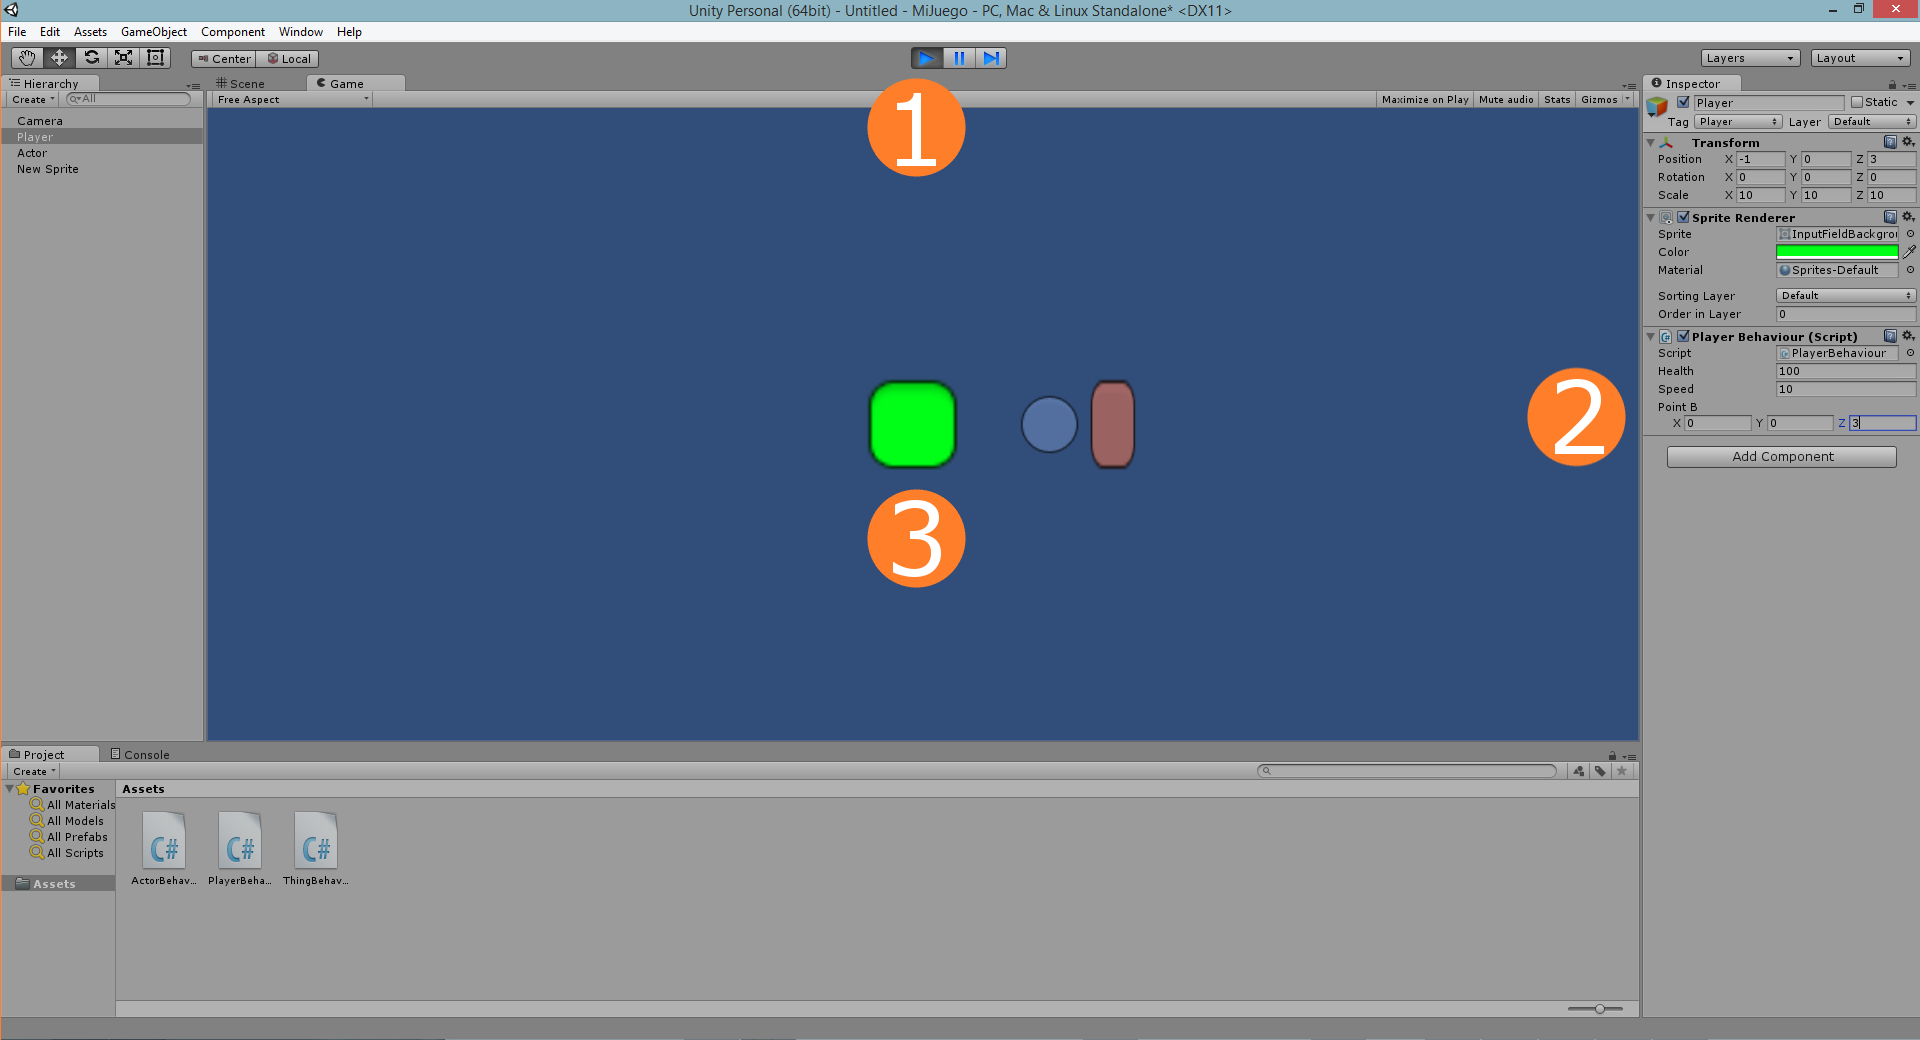
\includegraphics[width=0.80\linewidth]{media/1_ss8.jpg} 
\label{fig:unity_8}
\end{figure}

Otro requerimiento en la actividad consiste en implementar la cámara según el diseño del juego.

\begin{wrapfigure}[10]{l}{0.4\linewidth}
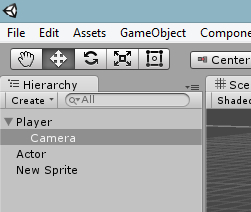
\includegraphics[width=\linewidth]{media/1_ss9.jpg} 
\end{wrapfigure}
En este ejemplo se asume una cámara seguidora tipo side-scroller. Esto es sumamente sencillo en Unity utilizando la jerarquía de objetos, para hacer a la transformada de \emph{Camera} dependiente de la transformada del \emph{Player} simplemente colocamos a \emph{Camera} como hijo del objeto \emph{Player}, para hacer esto realizamos click sostenido sobre el objeto \emph{Camera} en la jerarquía y lo colocamos sobre el objeto \emph{Player}. Ahora la cámara se mueve junto con el jugador.